\section{Visualisation}

Vast amounts of information is given to use on a daily basis. Everything from 
emails to credit card statements, from variations in the stock markets to the 
last-minute holiday offers, we are continuously bombarded with information.

All of the above examples have a common question that we subconsciously ask 
ourselves every time a new piece of information is obtained: Which email can 
can we delete because it doesn't interest us?  How much is outstanding upon 
the credit card? Do we need to cut back in the future? The common theme is
decision making.

We are not witnessing an explosion of information, but an explosion of data 
\citep{riccardo09}. It is this data that we are continuously trying to observe,
process and develop for everyday lives.

This leads to an interesting question, how is information created from data?

\citep{jacobson09} describes the process of understanding where data as the 
``continuum of understanding''. The continuum of understanding 
(Figure \ref{fig:datawisdom}), highlights how data can be transformed into 
information, and then into knowledge and ultimately wisdom.

\begin{figure}[H]
  \centering
    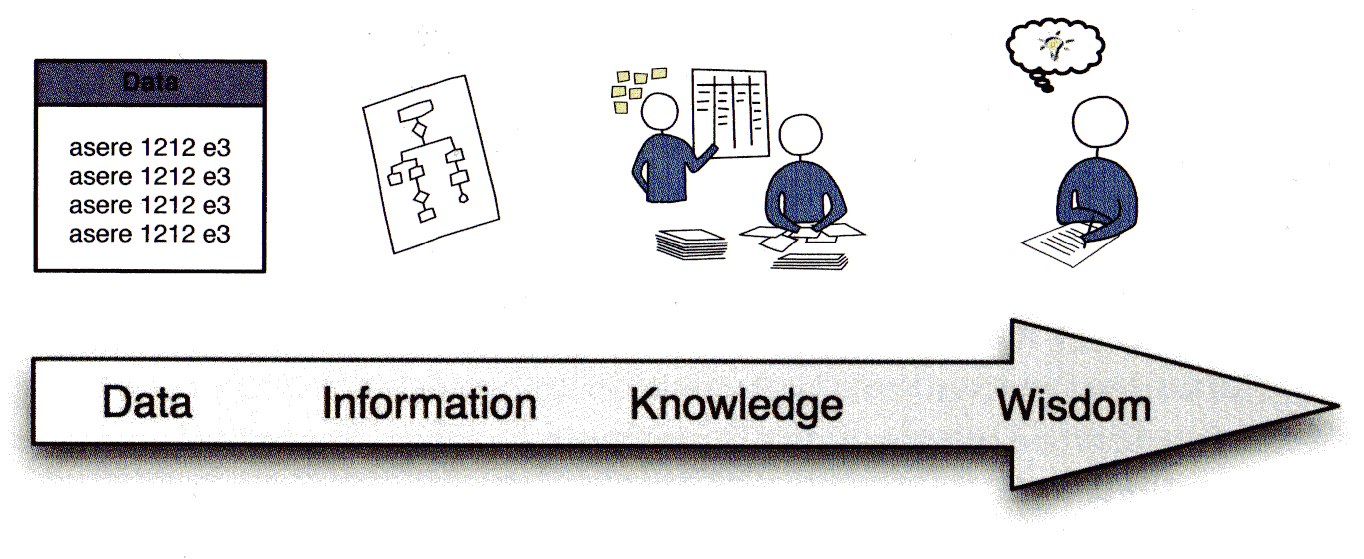
\includegraphics[scale=1.2]{chapter3/visualisation/data_wisdom.png}
  \label{fig:datawisdom}
  \caption[The continuum of understanding]
          {The continuum of understanding.}
\end{figure}

There are four main features within the process, as outlined below 
\citep{riccardo09}:
\begin{itemize}
  \item {\bf Data} are entities that have no meaning. They are the ``building 
        blocks'' of information.
  \item {\bf Information} provides meaning to data, by processing, organising, 
        and presenting in a suitable format.
  \item {\bf Knowledge} is the combination of information and experience. When 
        experiences are gained we are able to acquire the knowledge to help us 
        understand things.
  \item {\bf Wisdom} is the ``highest level of comprehension''. In order to 
        have wisdom, a person will have needed to have acquired such an 
        advanced level of knowledge.
\end{itemize}

Information visualisation is located between data and information, as it 
provides the methods to organise and represent the data, but does not provide 
any direct knowledge or wisdom acquisition \citep{riccardo09}. 

The remainder of this chapter will focus upon visualisation techniques.

% Graph Design
\subsection{Graph Design}

There are four `rules' to apply when choosing a graph format \citep{kosslyn06}.
If the wrong type of graph is chosen then the graph will not communicate with 
the reader effectively --- no matter how pretty it looks. 

The four `rules' are:
\begin{enumerate}
  \item Use a graph to illustrate relative amounts;
  \item Specify the subject;
  \item Present the data needed for a specific purpose;
  \item Use known concepts and formats.
\end{enumerate}


\subsubsection*{Illustrate}
A graph should only be used to illustrate relations amongst data 
\citep{kosslyn06} because graphs use variations within a visual dimension. This
allows us to recognise that one bar in a given bar chart is larger than another
bar in the same chart. 

\begin{quote}
  ``our perceptual systems allow us to quickly to detect difference among 
  heights, or the slope of lines. However, they do not allow us to register 
  absolute heights or slopes very well.'' \citep{kosslyn06}
\end{quote}

This is the fundamental reason, as to why graphs should illustrate the data, 
rather than allowing the reader to automatically obtain knowledge or wisdom.

In order to recognise specific values, the reader has to constantly refer back 
to the graph's scale, and make comparisons between each bar or slope. This 
will not only become annoying, but it will remove the focus from the data and 
towards the lesser important scale.


\subsubsection*{Specify}
In order for a reader to understand what the display is informing them of, they
need to know what it is the display is trying to inform them of 
\citep{kosslyn06}. This can be achieved by utilising a simple, precise, 
descriptive title.

Title of a display must be thought of before creating the display. This will 
help to decide what is useful and relevant within the display \citep{kosslyn06}.

An example could be ``Plant Productivity, 1995 -- 2000'', which would lead you 
to include data for each of the years, whereas a title such as ``Number of 
Units Produced in the United Kingdom'' would lead you to include data that is 
the average annual production figures for the United Kingdom.


\subsubsection*{Purpose}
A graph should allow people to answer specific questions. The nature of the 
question, and the information to answer that question needs to be specific 
\citep{kosslyn06}.

``People expect a question to be answered with the appropriate amount of 
information. No more and no less.'' \citep{grice75}. Readers use displays to 
answer questions, and require that there questions are answered in the context 
of the display. Hence why the display must have a purpose.


\subsubsection*{Formats}
``Displays are designed to communicate to a particular audience'' 
\citep{kosslyn06}. The concepts that are presented to the audience must be 
familiar and recognisable to the audience. Terminology, language and notations
must be followed within the display otherwise the audience may become confused.

Readers can only interpret a display if they have already stored the necessary
background in memory \citep{kosslyn06}.

Once the audience and the numbers that are to be displayed have been thought 
of, then the consideration of particular graphing formats can begin 
\citep{kosslyn06}. 

The chosen graph will depend upon the type of data that is being displayed. 
Within this section, a number of ``classic'' graphing displays will be 
discussed.


% Graph Variations
\subsection{Pie Graph}
``The most common way to display how a single whole is divided into parts is to
use a pie graph'' \citep{kosslyn06}. There are a number of `rules' to consider 
when using a pie graph.

\paragraph{Approximation} ~\\
A pie graph is excellent at conveying general information about proportions, 
but cannot display precise amounts such as a percentage of one part 
\citep{kosslyn06}.This information cannot be easily obtained, as readers find 
it hard to measure the angles and areas of pie charts precisely. 

Consider two parts if a pie chart that had a percentage of 35\% and 40\%. To 
the reader they would both appear to have the same area, even though their 
percentages differ. Figure \ref{fig:pieapprox} highlight this.

\begin{figure}[H]
  \centering
    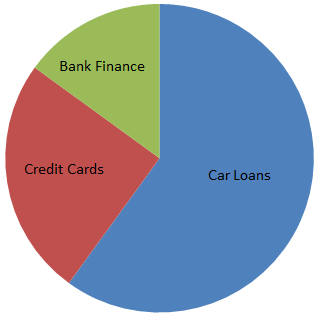
\includegraphics[scale=1]{chapter3/visualisation/pie_chart_approximate.png}
  \caption{Pie Chart with no size indicator.}
  \label{fig:pieapprox}
\end{figure}


\paragraph{Emphasize} ~\\
An exploded pie chart can be used to emphasize a small proportion of parts. 
This is achieved by displaying the important slice, as if it were a wedge of 
pizza being pulled out. 

Exploded pie charts can be effective because of the neurons in the visual 
system \citep{kosslyn06}. ``They can be thought of a difference detectors'', as
they respond most effectively to a change in a stimulation. The change can be
through colour or size. Figure \ref{fig:pieemphasis} highlights this.

\begin{figure}[H]
  \centering
    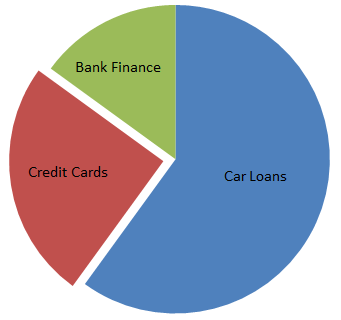
\includegraphics[scale=1]{chapter3/visualisation/pie_chart_emphasize.png}
  \caption{Pie Chart utilising emphasis.}
  \label{fig:pieemphasis}
\end{figure}


\subsection{Divided-Bar Graph}
A divided bar graph highlights the length of each segment within one bar. This 
effectively allows for smaller proportions to be combined together to form a 
larger dataset, and can allow for easy comparisons.

\paragraph{Accuracy} ~\\
Distance along a single extend is not distorted as area is by the visual system
\citep{kosslyn06}. This allows the reader to be able to extract precise amounts
in this format, however can cause confusion when trying to compare among 
values, as graph labels may loose their power of visual display.
Figure \ref{fig:dividedbar} highlights this.

\begin{figure}[H]
  \centering
    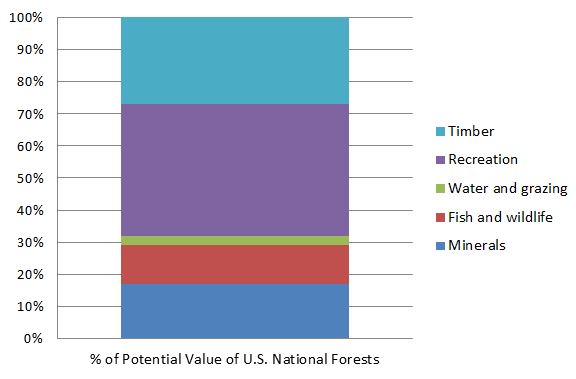
\includegraphics[scale=1]{chapter3/visualisation/divided_bar_graph.png}
  \caption{An example use of a divided-bar graph.}
  \label{fig:dividedbar}
\end{figure}


\subsection{Line and Bar Graph}
Line and Bar graphs are the most common formats used to display quantitative 
data, both in technical and popular media \citep{kosslyn06}. Both graphs are 
good at displaying changes over time.

\paragraph{Interactions} ~\\
Line graphs are better at displaying interactions between datasets. The reason 
for this is that the quantitative pattern is signalled directly by the visual 
patterns themselves \citep{kosslyn06}. Figure \ref{fig:line_bar_interactions}
highlights this.

\begin{figure}[H]
  \centering
    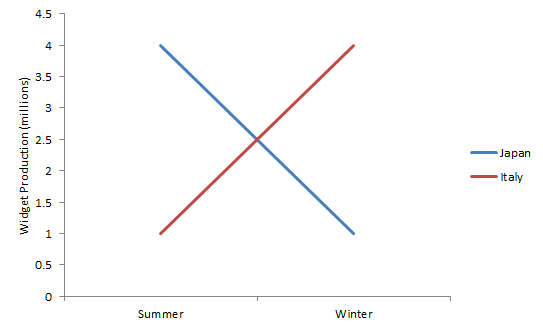
\includegraphics[scale=1]{chapter3/visualisation/line_bar_interactions.png}
  \caption{An example use of a line graph.}
  \label{fig:line_bar_interactions}
\end{figure}


\paragraph{Relative} ~\\
A bar graph should be used if the reader is supposed to compare specific 
measurements \citep{kosslyn06}. The reason for this is that the height of each 
bar specifies one point value, and thus increases the readability of the bar. 

When comparing to a line graph, the reader must locate and perceptually isolate
a point along the line \citep{kosslyn06}.

\begin{figure}[H]
  \centering
    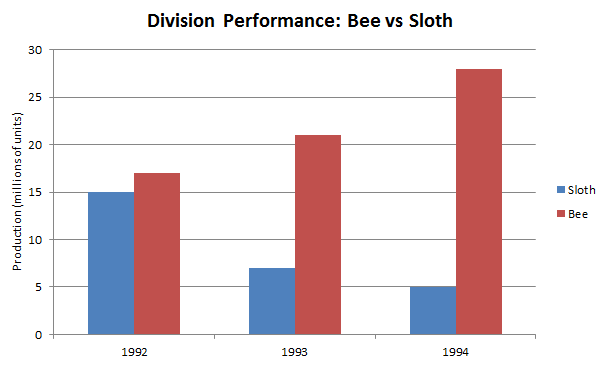
\includegraphics[scale=1]{chapter3/visualisation/line_bar_relative.png}
  \caption{An example use of a bar graph.}
  \label{fig:line_bar_relative}
\end{figure}


\paragraph{Horizontal or Vertical} ~\\
A horizontal bar-graph should be used if the data being displayed have a 
left-to-right or top-to-bottom order in the world. An example could be braking 
distances (Figure \ref{fig:line_bar_hori}).

However it must also be noted that a horizontal bar-graph should be used if the
labels are too long to fit under a vertical bar-graph --- as long as no other
recommendations are violated \citep{kosslyn06}.

``When in doubt, use a vertical bar-graph format'' \citep{kosslyn06}. The 
reason for this is that most people are used to a vertical bar-graph, and are 
able to discover trends easier with a vertical bar-graph in comparison to a 
horizontal bar-graph.

\begin{figure}[H]
  \centering
    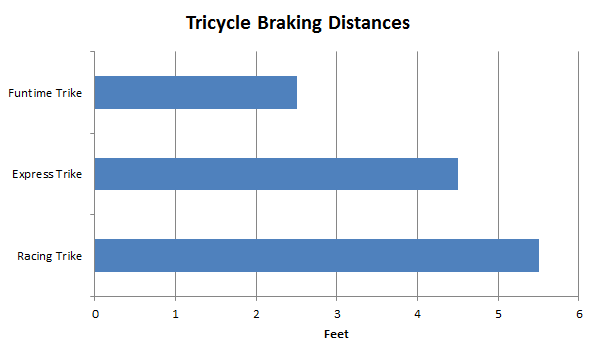
\includegraphics[scale=1]{chapter3/visualisation/line_bar_hori.png}
  \caption{An example use of a horizontal bar graph.}
  \label{fig:line_bar_hori}
\end{figure}


\subsection{Side-by-Side Graph}
A side-by-side graph shows pairs of values that share a central Y axis 
\citep{kosslyn06}. Upon the left hand side (of the centre) are measurements of
one variable, with the right-hand side exposing another variable.

\paragraph{Contrast} ~\\
A side-by-side graph highlights explicitly the relative patters over different 
level of a given variable. As the human visual system readily recognises 
differences, readers will be able to quickly determine the differences between 
a `regular' datum and an `irregular' datum \citep{kosslyn06}.

Side-by-side graphs allow for differences in their length to be instantaneously
recognised \citep{kosslyn06}. They allow for both contrasting of trends and but
also to flag specific differing values.

\paragraph{Importance} ~\\
A side-by-side graph can be used if comparisons between the individual pairs of 
values are most important \citep{kosslyn06}. As previously mentioned, 
side-by-side graphs allow for highlighting of contrasting of trends and the 
flagging of specific differing values.

\paragraph{Independent Variables} ~\\
Side-by-side graphs are excellent at contrasting on variable, and are not good 
at contrasting multiple variables \citep{kosslyn06}. 


\subsection{Step Graph}
Step graphs use lines as content element, but the lines trace out over 
horizontal plateaus \citep{kosslyn06}. Each plateaus can change height (much 
like a bar chart), but once pushed together they form a number of steps.

\paragraph{Trends} ~\\
Step graphs highlight noticeable changes over a number of values --- usually 
three or more values upon the X axis \citep{kosslyn06}. However, the values do
not vary continuously. By pushing each of the steps together it further 
highlights trends, and allows the reader to pick up on these trends at a glance
of the graph.

\paragraph{Multiple Variables} ~\\
A step graph makes it hard to distinguish between multiple variables, and 
multiple variables should not be shown upon the same graph \citep{kosslyn06}.


\subsection{Scatterplot}
Scatterplot graphs employ point symbols (such as dots, triangles and squares) 
as content elements, with the height of each point indicated by a given amount
\citep{kosslyn06}. 

It is more often than not that a scatterplot will look highly dense because of 
the number of points that are plotted, however they do have a number of 
advantages.

\paragraph{Impressions} ~\\
Scatterplots allow readers to gain an overall impression of the relation of two
variables \citep{kosslyn06}. An example could be the plotting of people's 
heights and weights, as show in figure \ref{fig:scatterplot_line}.

\begin{figure}[H]
  \centering
    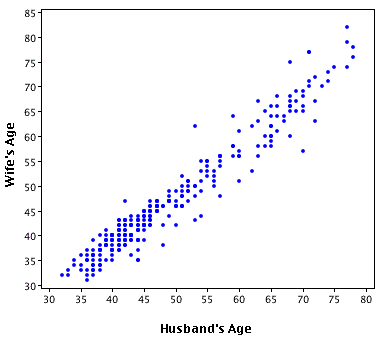
\includegraphics[scale=1]{chapter3/visualisation/scatterplot.png}
  \caption{An example use of a scatterplot.}
  \label{fig:scatterplot_line}
\end{figure}


\paragraph{Relations} ~\\
Scatterplots are used to illustrate a trend, which can be summarised by a line
\citep{kosslyn06}. This line is a fitted line, as it does not connect the 
points, it simply highlights the trend for a given set of data. It should fall
through the centre of the most populated area \citep{kosslyn06}.

Figure \ref{fig:scatterplot_line} illustrates an example scatterplot with a 
relationship line.

\begin{figure}[H]
  \centering
    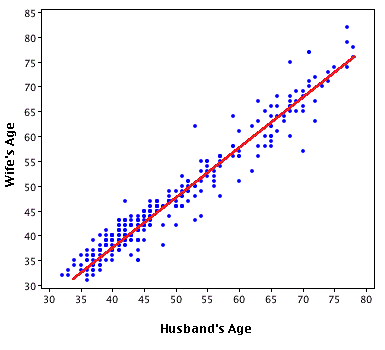
\includegraphics[scale=1]{chapter3/visualisation/scatterplot_line.png}
  \caption{An example use of a scatterplot with a trend line.}
  \label{fig:scatterplot_line}
\end{figure}


\subsection{Stacked Bars}
Stacked-bars consist of two or more parts, each specifying the value of a 
different level of the independent variable \citep{kosslyn06}. 

Stacked bars are most effective when illustrating components of wholes that 
change. Stack-bar graphs generally tend to follow the same properties as 
divided-bar graphs.

\paragraph{Nominal Scale} ~\\
Unlike a divided-bar graph, the overall height of the stack bar within a 
stack-bar graph can vary. This illustrates the use of two or more independent 
variables \citep{kosslyn06}. Figure \ref{fig:stacked_bars} highlights the use
of a stacked bar.

\begin{figure}[H]
  \centering
    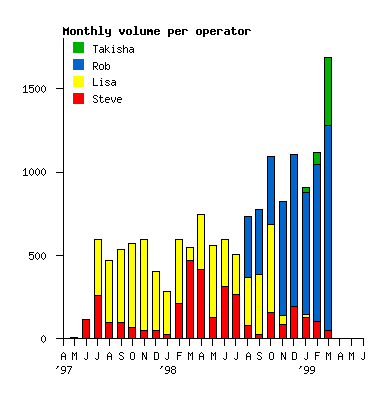
\includegraphics[scale=1]{chapter3/visualisation/stacked_bars.png}
  \caption{An example use of a stacked bar.}
  \label{fig:stacked_bars}
\end{figure}


\subsection{Optional Features}
In order to improve general readability, a number of additional features can be
added to almost any graph \citep{kosslyn06}. These are:
\begin{itemize}
  \item Use a key when direct labels can not be used;
  \item Consider using error bars when error margins are known;
  \item Use an inner grid when precise values are important;
  \item Do not use mixed bar/line displays to show interactions;
  \item Include a caption to clarify unfamiliar terms.
\end{itemize}
